% 20120511-123824-124126
% A-6.6/W22.1

\section{A-6.6/W22.1 - 160 krpm}
\label{sec:awp-exp-details-A-6.6/W22.1}

This test has been performed on May 11\th{} 2012, between 12:38:24 and
12:41:26.

\begin{figure}[htbp]
  \centering
  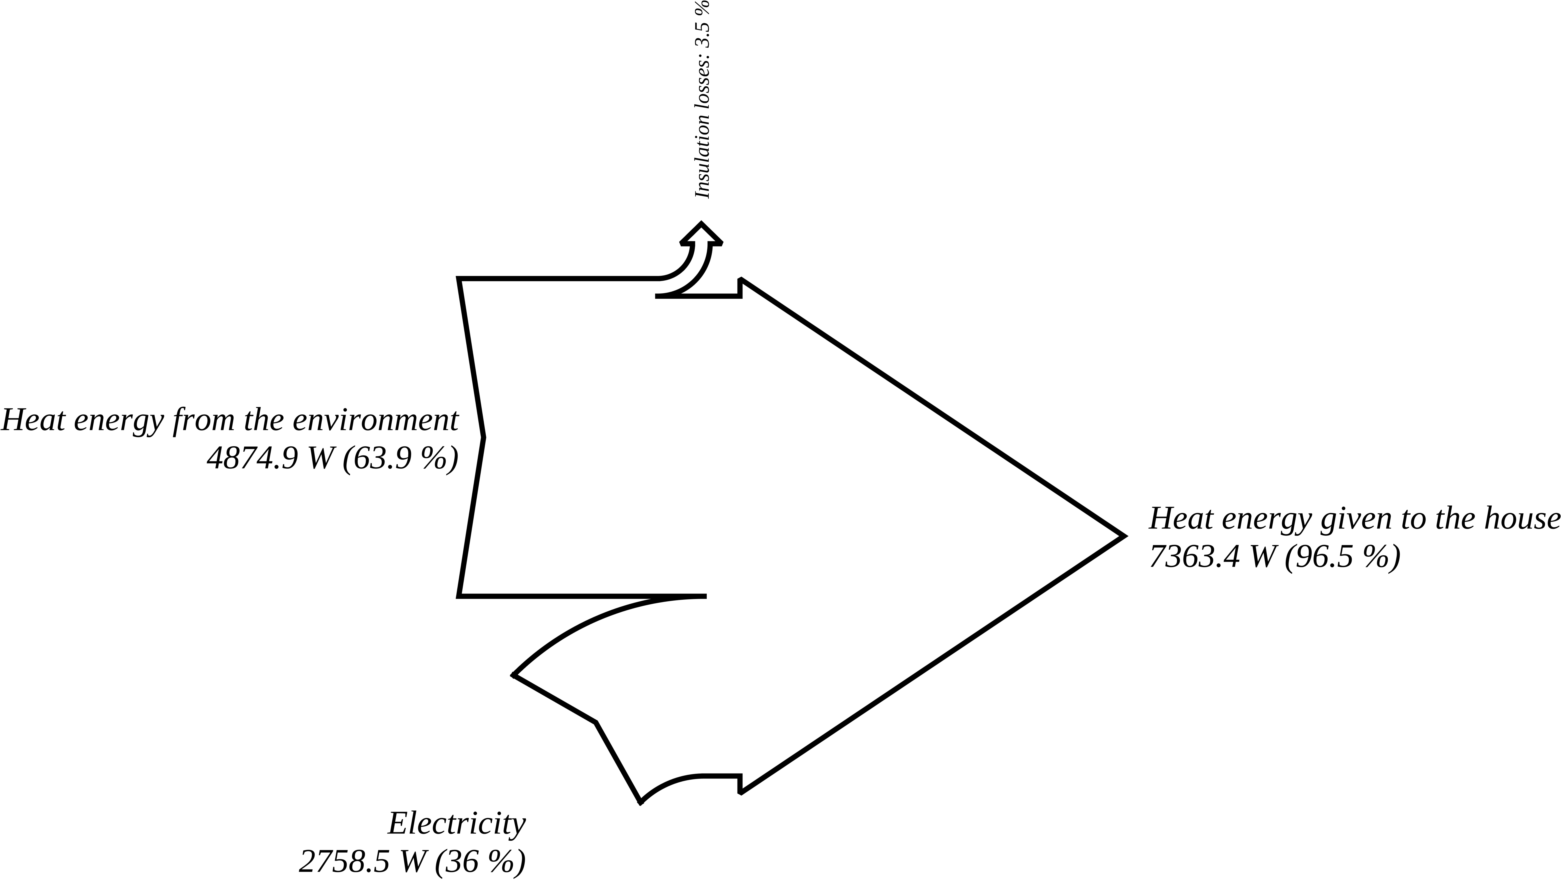
\includegraphics[width=0.7\textwidth]{awp-energy-sankey-awp-20120511-123824-124126}
  \caption{A-6.6/W22.1 -- Sankey diagram for heat pump energy balance (internal frontier)}
  \label{fig:awp-A-6.6/W22.1-sankey-energy}
\end{figure}


\begin{figure}[htbp]
  \centering
  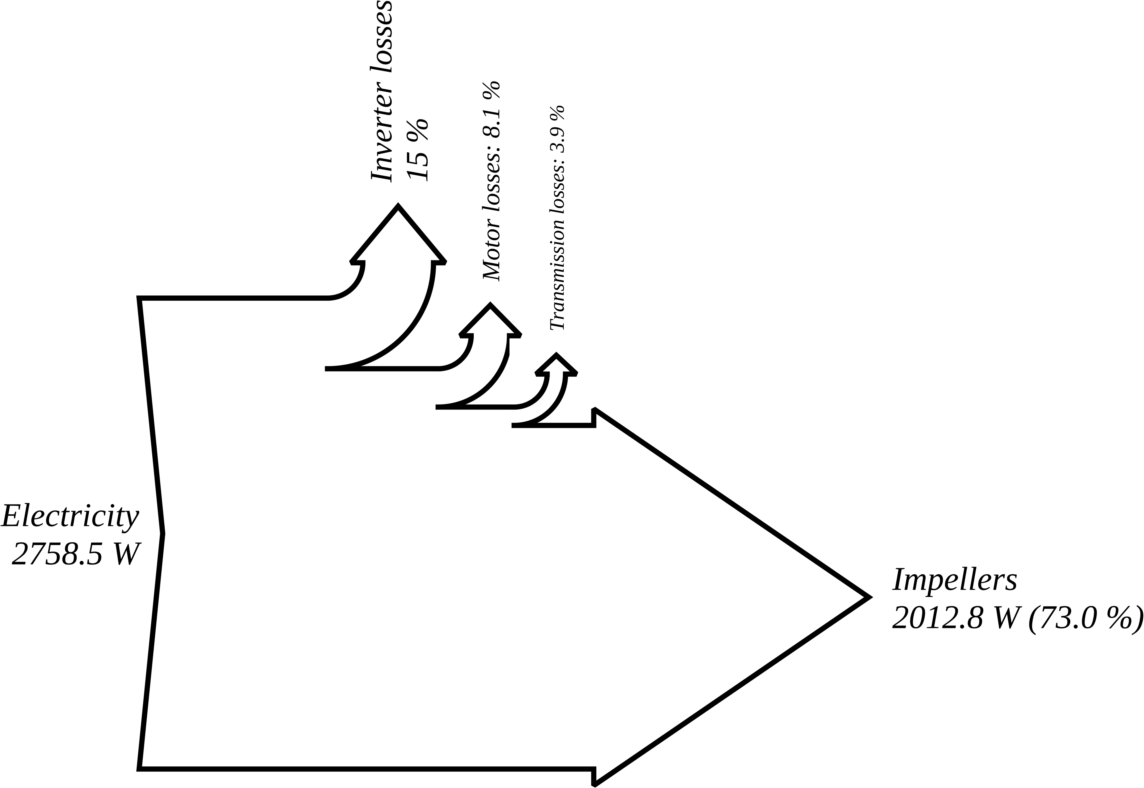
\includegraphics[width=0.7\textwidth]{awp-energy-sankey-cp-20120511-123824-124126}
  \caption{A-6.6/W22.1 -- Sankey diagram for the compressor unit energy balance}
  \label{fig:awp-A-6.6/W22.1-sankey-cp}
\end{figure}

\begin{figure}[htbp]
  \centering
  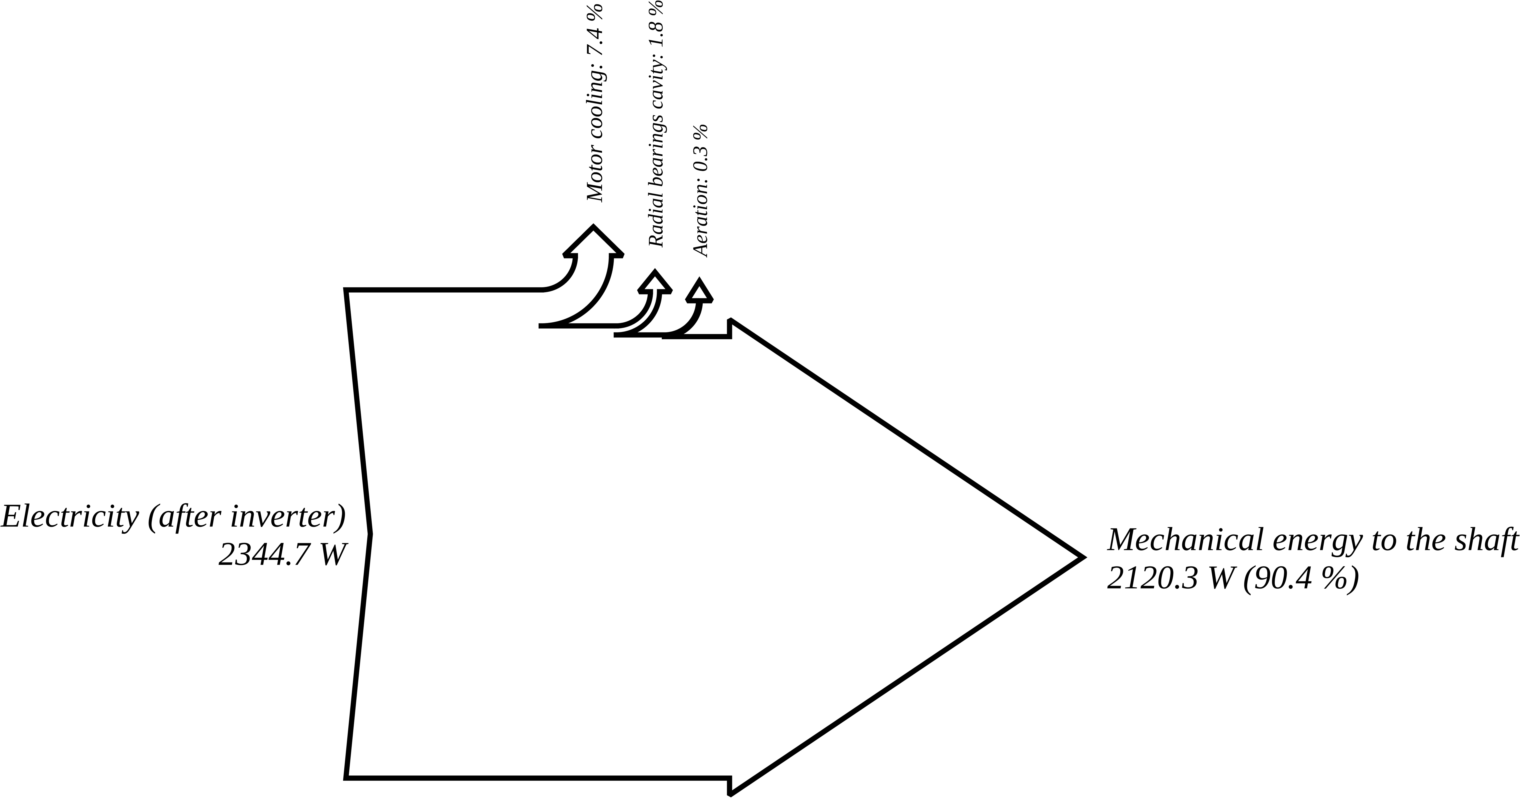
\includegraphics[width=0.7\textwidth]{awp-energy-sankey-motor-20120511-123824-124126}
  \caption{A-6.6/W22.1 -- Sankey diagram for the motor energy balance}
  \label{fig:awp-A-6.6/W22.1-sankey-motor}
\end{figure}

\begin{table}[htbp]
    \footnotesize
    \begin{center}
    \begin{tabular}{llllll}
\toprule
Name & Value / \% & Name & Value / \% & Name & Value / - \\
\midrule
$\eta_{heatpump}$ & $ \num{25.2} \pm \num{0.7} $ & $\eta_{motor}$ & $ \num{90.35} \pm \num{0.09} $ & $\epsilon_h$ & $ \num{2.67} \pm \num{2.67} $\\
$\eta_{cp1}$ & $ \num{74} \pm \num{26} $ & $\eta_{cp2}$ &$ \num{54} \pm \num{27} $ & $\pi_1$ & $ \num{2.511} \pm \num{2.511} $\\
$\eta_{cp1,\,imp}$ & $ \num{71} \pm \num{30} $ & $\eta_{cp2,\,imp}$ & $ \num{60} \pm \num{30} $ & $\pi_2$ & $ \num{2.375} \pm \num{2.375} $\\
$\eta_{cd}$ & $ \num{93} \pm \num{4} $ & $\eta_{ev}$ & $ \num{30} \pm \num{30} $ & $\pi_{1,\,theory}$ & $ \num{3.2} \pm \num{3.2} $\\
$\eta_{trans}$ & $ \num{94.93} \pm \num{0.02} $ & $\eta_{sc}$ & $ \num{0.4} \pm \num{0.4} $ & $\pi_{2,\,theory}$ & $ \num{1.938} \pm \num{1.938} $\\
$\eta_{s,\,cp1}$ & $ \num{93} \pm \num{7} $ & $\eta_{s,\,cp2}$ & $ \num{86} \pm \num{13} $ & $\eta_{motor}$ & $\underline{90.43}$ \%\\
$\eta_{s,\,cp1,\,ext}$ & $ \num{98} \pm \num{2} $ & $\eta_{s,\,cp2,\,ext}$ & $ \num{47} \pm \num{47} $ & $\eta_{radial}$ & $ \num{98.13} \pm \num{0.02} $ \%\\
$\eta_{s,\,cp1,\,theory}$ & $ \num{78.4} \pm \num{0.3} $ & $\eta_{s,\,cp2,\,theory}$ & $ \num{73.00} \pm \num{0.05} $ & $\eta_{axial}$ & $ \num{96.74} \pm \num{0.02} $ \%\\
\bottomrule
\end{tabular}

  \end{center}
  \caption{A-6.6/W22.1 -- Performance indicators}
\end{table}

\begin{table}[htbp]
  \footnotesize
  \begin{center}
    \begin{tabular}{cccccc}
\toprule
Component & Location & P / \si{\bar} & T / \si{\degreeCelsius} & h / \si{\kilo\joule\per\kilo\gram} & s / \si{\kilo\joule\per\kilo\gram\per\kelvin}\\
\midrule
\multirow{2}{*}{1} & inlet & $ \num{1.077} \pm \num{0.001} $ & $ \num{-12} \pm \num{13} $ & $ \num{393.55} \pm \num{0.02} $ & $ \num{1.78} \pm \num{0.04} $\\
& outlet & $ \num{2.704} \pm \num{0.001} $ & $ \num{26} \pm \num{3} $ & $ \num{422.594} \pm \num{0.003} $ & $ \num{1.82} \pm \num{0.01} $\\
\midrule
\multirow{2}{*}{2} & inlet & $\pmb{ \num{2.704} \pm \num{0.001} }$ & $\pmb{ \num{4.176} \pm \num{0.007} }$ & $ \num{402.939191} \pm \num{7e-06} $ & $ \num{1.74878} \pm \num{8e-05} $\\
& outlet & $\pmb{ \num{6.423} \pm \num{0.001} }$ & $\pmb{ \num{38.933} \pm \num{0.007} }$ & $ \num{426.842379} \pm \num{7e-06} $ & $ \num{1.76628} \pm \num{5e-05} $\\
\midrule
\multirow{2}{*}{3} & inlet & $\pmb{ \num{6.291} \pm \num{0.001} }$ & $\pmb{ \num{34.209} \pm \num{0.005} }$ & $ \num{422.462530} \pm \num{5e-06} $ & $ \num{1.75362} \pm \num{4e-05} $\\
& outlet & $\pmb{ \num{6.083} \pm \num{0.001} }$ & $\pmb{ \num{19.689} \pm \num{0.005} }$ & $ \num{227.034683} \pm \num{5e-06} $ & $ \num{1.09466} \pm \num{3e-05} $\\
\midrule
\multirow{2}{*}{4} & inlet & $ \num{1.674} \pm \num{0.001} $ & $ \num{-14.5} \pm \num{0.8} $ & $ \num{211.4870} \pm \num{8e-04} $ & $ \num{1.047} \pm \num{0.003} $\\
& outlet & $\pmb{ \num{1.632} \pm \num{0.001} }$ & $\pmb{ \num{-14.818} \pm \num{0.005} }$ & $ \num{389.804601} \pm \num{5e-06} $ & $ \num{1.7381} \pm \num{1e-04} $\\
\midrule
\multirow{2}{*}{5} & inlet & $ \num{6.083} \pm \num{0.001} $ & $ \num{19.69} \pm \num{0.04} $ & $ \num{227.03468} \pm \num{4e-05} $ & $ \num{1.0947} \pm \num{2e-04} $\\
& outlet & $ \num{2.704} \pm \num{0.001} $ & $ \num{-2.2} \pm \num{0.6} $ & $ \num{227.0347} \pm \num{6e-04} $ & $ \num{1.100} \pm \num{0.002} $\\
\midrule
\multirow{2}{*}{6} & inlet & $ \num{2.704} \pm \num{0.001} $ & $ \num{-5} \pm \num{8} $ & $ \num{193.444} \pm \num{0.008} $ & $ \num{0.98} \pm \num{0.04} $\\
& outlet & $ \num{1.843} \pm \num{0.001} $ & $ \num{-12.1} \pm \num{0.7} $ & $ \num{193.4444} \pm \num{7e-04} $ & $ \num{0.977} \pm \num{0.004} $\\
\midrule
\multirow{2}{*}{7} & inlet & $ \num{1.843} \pm \num{0.001} $ & $ \num{-12.1} \pm \num{0.7} $ & $ \num{227.0347} \pm \num{7e-04} $ & $ \num{1.105} \pm \num{0.003} $\\
& outlet & $ \num{1.843} \pm \num{0.001} $ & $ \num{36} \pm \num{11} $ & $ \num{432.54} \pm \num{0.02} $ & $ \num{1.88} \pm \num{0.03} $\\
\midrule
\multirow{2}{*}{8} & inlet & $\pmb{ \num{2.704} \pm \num{0.001} }$ & $\pmb{ \num{-2.173} \pm \num{0.007} }$ & $ \num{397.330155} \pm \num{7e-06} $ & $ \num{1.72832} \pm \num{2e-05} $\\
& outlet & $ \num{2.70} \pm \num{0.06} $ & $ \num{-2.2} \pm \num{0.6} $ & $ \num{197.0870} \pm \num{6e-04} $ & $ \num{0.989} \pm \num{0.003} $\\
\midrule
\multirow{2}{*}{9} & inlet & $\pmb{ \num{1.843} \pm \num{0.001} }$ & $\pmb{ \num{-12.131} \pm \num{0.005} }$ & $ \num{211.486983} \pm \num{5e-06} $ & $ \num{1.04571} \pm \num{8e-05} $\\
& outlet & $ \num{1.674} \pm \num{0.001} $ & $ \num{-14.5} \pm \num{0.8} $ & $ \num{211.4870} \pm \num{8e-04} $ & $ \num{1.047} \pm \num{0.003} $\\
\midrule
\multirow{2}{*}{10} & inlet & $ \num{6.423} \pm \num{0.001} $ & $ \num{39} \pm \num{3} $ & $ \num{426.842} \pm \num{0.003} $ & $ \num{1.766} \pm \num{0.008} $\\
& outlet & $ \num{2.704} \pm \num{0.001} $ & $ \num{135} \pm \num{98} $ & $ \num{526.2} \pm \num{0.1} $ & $ \num{2.1} \pm \num{0.2} $\\
\midrule
\multirow{2}{*}{11} & inlet & $ \num{1.077} \pm \num{0.001} $ & $ \num{104} \pm \num{46} $ & $ \num{496.09} \pm \num{0.05} $ & $ \num{2.1} \pm \num{0.1} $\\
& outlet & $ \num{1.077} \pm \num{0.001} $ & $ \num{117} \pm \num{55} $ & $ \num{509.36} \pm \num{0.06} $ & $ \num{2.1} \pm \num{0.1} $\\
\midrule
\multirow{2}{*}{12} & inlet & $ \num{1.466} \pm \num{0.001} $ & $ \num{16} \pm \num{33} $ & $ \num{415.90} \pm \num{0.04} $ & $ \num{1.8} \pm \num{0.1} $\\
& outlet & $ \num{1.466} \pm \num{0.001} $ & $ \num{39} \pm \num{38} $ & $ \num{436.10} \pm \num{0.04} $ & $ \num{1.9} \pm \num{0.1} $\\
\midrule
\multirow{2}{*}{13} & inlet & $ \num{1.466} \pm \num{0.001} $ & $ \num{8} \pm \num{4} $ & $ \num{409.132} \pm \num{0.004} $ & $ \num{1.82} \pm \num{0.01} $\\
& outlet & $ \num{1.466} \pm \num{0.001} $ & $ \num{17} \pm \num{34} $ & $ \num{416.65} \pm \num{0.04} $ & $ \num{1.8} \pm \num{0.1} $\\
\midrule
\multirow{2}{*}{15} & inlet & & $\pmb{ \num{17.061} \pm \num{0.005} }$ & \multicolumn{2}{l}{Cp = $ \num{4186.081} \pm \num{0.005} $ \si{\joule\per\kilo\gram\per\kelvin}}\\
& outlet & & $\pmb{ \num{22.097} \pm \num{0.005} }$ & \multicolumn{2}{l}{Cp = $ \num{4182.430} \pm \num{0.004} $ \si{\joule\per\kilo\gram\per\kelvin}}\\
\midrule
\multirow{2}{*}{16} & inlet & & $\pmb{ \num{-6.647} \pm \num{0.005} }$ & & \\
& outlet & & $\pmb{ \num{-10.248} \pm \num{0.005} }$ & & \\
\midrule
\multirow{2}{*}{18} & inlet & $ \num{1.632} \pm \num{0.001} $ & $ \num{-14.8} \pm \num{0.5} $ & $ \num{389.8046} \pm \num{5e-04} $ & $ \num{1.738} \pm \num{0.003} $\\
& outlet & $\pmb{ \num{1.077} \pm \num{0.001} }$ & $\pmb{ \num{-21.08} \pm \num{0.01} }$ & $ \num{386.53683} \pm \num{1e-05} $ & $ \num{1.7575} \pm \num{2e-04} $\\
\midrule
\multirow{2}{*}{19} & inlet & $ \num{2.704} \pm \num{0.001} $ & $ \num{-2.2} \pm \num{0.6} $ & $ \num{197.0870} \pm \num{6e-04} $ & $ \num{0.989} \pm \num{0.003} $\\
& outlet & $ \num{2.704} \pm \num{0.001} $ & $ \num{-5} \pm \num{8} $ & $ \num{193.444} \pm \num{0.008} $ & $ \num{0.98} \pm \num{0.04} $\\
\midrule
\multirow{2}{*}{20} & inlet & $ \num{6.423} \pm \num{0.001} $ & $ \num{39} \pm \num{3} $ & $ \num{426.842} \pm \num{0.003} $ & $ \num{1.766} \pm \num{0.008} $\\
& outlet & $ \num{6.291} \pm \num{0.001} $ & $ \num{34} \pm \num{3} $ & $ \num{422.463} \pm \num{0.003} $ & $ \num{1.754} \pm \num{0.009} $\\
\midrule
\multirow{2}{*}{21} & inlet & $ \num{1.466} \pm \num{0.001} $ & $ \num{8} \pm \num{4} $ & $ \num{409.132} \pm \num{0.004} $ & $ \num{1.82} \pm \num{0.01} $\\
& outlet & $\pmb{ \num{1.494} \pm \num{0.001} }$ & $\pmb{ \num{7.857} \pm \num{0.007} }$ & $ \num{409.068827} \pm \num{7e-06} $ & $ \num{1.8165} \pm \num{1e-04} $\\
\midrule
\multirow{2}{*}{22} & inlet & $ \num{1.077} \pm \num{0.001} $ & $ \num{-15} \pm \num{10} $ & $ \num{391.28} \pm \num{0.01} $ & $ \num{1.78} \pm \num{0.03} $\\
& outlet & $\pmb{ \num{1.077} \pm \num{0.001} }$ & $\pmb{ \num{-15.148} \pm \num{0.007} }$ & $ \num{391.282690} \pm \num{7e-06} $ & $ \num{1.7761} \pm \num{1e-04} $\\
\midrule
\multirow{2}{*}{23} & inlet & $ \num{1.077} \pm \num{0.001} $ & $ \num{117} \pm \num{55} $ & $ \num{509.36} \pm \num{0.06} $ & $ \num{2.1} \pm \num{0.1} $\\
& outlet & $ \num{1.077} \pm \num{0.001} $ & $ \num{131} \pm \num{64} $ & $ \num{523.19} \pm \num{0.07} $ & $ \num{2.2} \pm \num{0.2} $\\
\midrule
\multirow{2}{*}{24} & inlet & $ \num{1.077} \pm \num{0.001} $ & $ \num{39} \pm \num{39} $ & $ \num{436.10} \pm \num{0.04} $ & $ \num{1.9} \pm \num{0.1} $\\
& outlet & $ \num{1.077} \pm \num{0.001} $ & $ \num{104} \pm \num{46} $ & $ \num{496.09} \pm \num{0.05} $ & $ \num{2.1} \pm \num{0.1} $\\
\midrule
\multirow{2}{*}{25} & inlet & $ \num{2.704} \pm \num{0.001} $ & $ \num{26} \pm \num{29} $ & $ \num{437.00} \pm \num{0.03} $ & $ \num{1.86} \pm \num{0.08} $\\
& outlet & $\pmb{ \num{2.704} \pm \num{0.001} }$ & $\pmb{ \num{42.561} \pm \num{0.007} }$ & $ \num{437.003251} \pm \num{7e-06} $ & $ \num{1.86379} \pm \num{7e-05} $\\
\midrule
\multirow{2}{*}{26} & inlet & $ \num{6.423} \pm \num{0.001} $ & $ \num{39} \pm \num{3} $ & $ \num{426.842} \pm \num{0.003} $ & $ \num{1.766} \pm \num{0.008} $\\
& outlet & $\pmb{ \num{1.466} \pm \num{0.001} }$ & $\pmb{ \num{7.857} \pm \num{0.007} }$ & $ \num{409.132471} \pm \num{7e-06} $ & $ \num{1.8182} \pm \num{1e-04} $\\
\midrule
\multirow{2}{*}{27} & inlet & $ \num{2.704} \pm \num{0.001} $ & $ \num{26} \pm \num{3} $ & $ \num{422.595} \pm \num{0.003} $ & $ \num{1.82} \pm \num{0.01} $\\
& outlet & $ \num{2.704} \pm \num{0.001} $ & $ \num{26} \pm \num{3} $ & $ \num{422.595} \pm \num{0.003} $ & $ \num{1.82} \pm \num{0.01} $\\
\midrule
\multirow{2}{*}{28} & inlet & $ \num{2.704} \pm \num{0.001} $ & $ \num{-2.2} \pm \num{0.4} $ & $ \num{397.3302} \pm \num{4e-04} $ & $ \num{1.728} \pm \num{0.001} $\\
& outlet & $ \num{2.704} \pm \num{0.001} $ & $ \num{4} \pm \num{4} $ & $ \num{402.939} \pm \num{0.004} $ & $ \num{1.75} \pm \num{0.01} $\\
\midrule
\multirow{2}{*}{29} & inlet & $ \num{1.077} \pm \num{0.001} $ & $ \num{-20} \pm \num{5} $ & $ \num{387.589} \pm \num{0.005} $ & $ \num{1.76} \pm \num{0.02} $\\
& outlet & $ \num{1.077} \pm \num{0.001} $ & $ \num{-14} \pm \num{11} $ & $ \num{391.96} \pm \num{0.02} $ & $ \num{1.78} \pm \num{0.04} $\\
\bottomrule
\end{tabular}

  \end{center}
  \caption{A-6.6/W22.1 -- Thermodynamic points of the heat pump cycle}
\end{table}


\begin{table}[htbp]
    \footnotesize
    \begin{center}
    \begin{tabular}{llllll}
\toprule
Name & Value / \si{\gram\per\second} & Name & Value / \si{\gram\per\second} & Name & Value / \si{\gram\per\second} \\
\midrule
$\dot{M}_{1 \rightarrow 25}$ & $ \num{23} \pm \num{1} $ & $\dot{M}_{2 \rightarrow 10}$ & $\underline{3.66}$ & $\dot{M}_{2 \rightarrow 20}$ & $ \num{37.7} \pm \num{0.8} $ \\
$\dot{M}_{2 \rightarrow 26}$ & $\pmb{ \num{1.20} \pm \num{0.06} }$ & $\dot{M}_{3 \rightarrow 5}$ & $ \num{35.5} \pm \num{0.8} $ & $\dot{M}_{3 \rightarrow 7}$ & $\pmb{ \num{2.21} \pm \num{0.03} }$ \\
$\dot{M}_{4 \rightarrow 18}$ & $ \num{21} \pm \num{1} $ & $\dot{M}_{5 \rightarrow 8}$ & $ \num{35.5} \pm \num{0.8} $ & $\dot{M}_{6 \rightarrow 9}$ & $ \num{19} \pm \num{1} $ \\
$\dot{M}_{7 \rightarrow 9}$ & $ \num{2.21} \pm \num{0.03} $ & $\dot{M}_{8 \rightarrow 19}$ & $ \num{19} \pm \num{1} $ & $\dot{M}_{8 \rightarrow 28}$ & $ \num{33} \pm \num{2} $ \\
$\dot{M}_{9 \rightarrow 4}$ & $ \num{21} \pm \num{1} $ & $\dot{M}_{10 \rightarrow 25}$ & $3.66$ & $\dot{M}_{11 \rightarrow 22}$ & $ \num{0.36} \pm \num{0.02} $ \\
$\dot{M}_{11 \rightarrow 23}$ & $ \num{0.84} \pm \num{0.04} $ & $\dot{M}_{12 \rightarrow 24}$ & $ \num{1.20} \pm \num{0.05} $ & $\dot{M}_{13 \rightarrow 12}$ & $ \num{1.08} \pm \num{0.05} $ \\
$\dot{M}_{17 \rightarrow 15}$ & $\pmb{ \num{368} \pm \num{5} }$ & $\dot{M}_{18 \rightarrow 22}$ & $ \num{21} \pm \num{1} $ & $\dot{M}_{19 \rightarrow 6}$ & $ \num{19} \pm \num{1} $ \\
$\dot{M}_{20 \rightarrow 3}$ & $ \num{37.7} \pm \num{0.8} $ & $\dot{M}_{21 \rightarrow 12}$ & $ \num{0.119} \pm \num{0.006} $ & $\dot{M}_{22 \rightarrow 29}$ & $ \num{22} \pm \num{1} $ \\
$\dot{M}_{23 \rightarrow 29}$ & $ \num{0.84} \pm \num{0.04} $ & $\dot{M}_{24 \rightarrow 11}$ & $ \num{1.20} \pm \num{0.05} $ & $\dot{M}_{25 \rightarrow 8}$ & $ \num{16.9} \pm \num{0.6} $ \\
$\dot{M}_{25 \rightarrow 27}$ & $ \num{9.4} \pm \num{0.4} $ & $\dot{M}_{26 \rightarrow 13}$ & $ \num{1.08} \pm \num{0.05} $ & $\dot{M}_{26 \rightarrow 21}$ & $ \num{0.119} \pm \num{0.006} $ \\
$\dot{M}_{27 \rightarrow 28}$ & $ \num{9.4} \pm \num{0.4} $ & $\dot{M}_{28 \rightarrow 2}$ & $ \num{43} \pm \num{2} $ & $\dot{M}_{29 \rightarrow 1}$ & $ \num{23} \pm \num{1} $ \\
$\dot{M}_{cp_1}$ & $ \num{23} \pm \num{1} $ & $\dot{M}_{cp_2}$ & $ \num{42.5} \pm \num{0.8} $ \\
\bottomrule
\end{tabular}

  \end{center}
  \caption{A-6.6/W22.1 -- Mass flow rates between the components}
\end{table}

\begin{table}[htbp]
    \footnotesize
    \begin{center}
    \begin{tabular}{llll}
\toprule
Name & Value / $W$ & Name & Value / $W$ \\
\midrule
$\dot{E}_{1 \rightarrow 2}$ & $ \num{1354} \pm \num{659} $ & $\dot{E}_{11 \rightarrow 1}$ & $ \num{2012.8} \pm \num{0.3} $ \\
$\dot{E}_{12 \rightarrow 11}$ & $ \num{2080.6} \pm \num{0.3} $ & $\dot{E}_{13 \rightarrow 12}$ & $ \num{2120.3} \pm \num{0.3} $ \\
$\dot{E}_{14 \rightarrow 13}$ & $ \num{2344.7} \pm \num{0.4} $ & $\dot{E}_{el \rightarrow 14}$ & $\pmb{ \num{2758.5} \pm \num{0.4} }$ \\
$\dot{Y}_{1 \rightarrow 2}$ & $ \num{27} \pm \num{27} $ & $\dot{Y}_{2 \rightarrow 10}$ & $ \num{364} \pm \num{364} $ \\
$\dot{Y}_{3 \rightarrow 15}$ & $ \num{7363} \pm \num{125} $ & $\dot{Y}_{11 \rightarrow 1}$ & $ \num{27} \pm \num{27} $ \\
$\dot{Y}_{11 \rightarrow 23}$ & $ \num{12} \pm \num{12} $ & $\dot{Y}_{11 \rightarrow 24}$ & $ \num{72} \pm \num{72} $ \\
$\dot{Y}_{12 \rightarrow 11}$ & $ \num{59} \pm \num{59} $ & $\dot{Y}_{13 \rightarrow 7}$ & $ \num{172.96} \pm \num{0.03} $ \\
$\dot{Y}_{13 \rightarrow 12}$ & $ \num{43.373} \pm \num{0.006} $ & $\dot{Y}_{14 \rightarrow at}$ & $ \num{413.78} \pm \num{0.06} $ \\
$\dot{Y}_{16 \rightarrow 4}$ & $ \num{4875} \pm \num{174} $ & $\dot{Y}_{19 \rightarrow 18}$ & $ \num{70} \pm \num{64} $ \\
$\dot{Y}_{20 \rightarrow at}$ & $ \num{165} \pm \num{120} $ & $\dot{Y}_{21 \rightarrow at}$ & $ \num{0.008} \pm \num{0.008} $ \\
$\dot{Y}_{26 \rightarrow at}$ & $ \num{21} \pm \num{5} $ \\
\bottomrule
\end{tabular}

  \end{center}
  \caption{A-6.6/W22.1 -- Energy rates between the components}
\end{table}

\FloatBarrier
